\documentclass[a4paper,11pt]{article}

\usepackage{a4wide}
\usepackage{epsfig}
\usepackage{dcolumn}
\usepackage{float}
\psfigdriver{dvips}

\begin{document}

\title{Comparing several Orca implementations using \\
the Arc Consistency Problem}
\author{R. van der Pol \\
rvdp{\tt @}cs.vu.nl \\ \\
Department of Mathematics and Computer Science \\
Vrije Universiteit \\
Amsterdam \\
The Netherlands}
\date{August 1995}

\maketitle

\begin{abstract}
Orca is a Modula-2 like programming language for writing parallel programs.
It is designed to be a portable language.  Its main 
paradigm for writing parallel programs is its shared data-object model.
A program which solves the arc consistency problem
was written in Orca
and was used to compare the performance
of three platforms (Amoeba on a collection of microSPARC processors
connected through an Ethernet,
Solaris on a group of microSPARC workstations connected through an Ethernet,
and Parix on a grid of PowerPCs connected with point to point links).
The measurements show good speedups on all of these platforms.
Because it is relatively easy to program in Orca it is an attractive
language to write parallel programs in.
\end{abstract}

\section{Introduction}

In recent years more and more computer
manufacturers produce multiprocessor systems, because it becomes increasingly
difficult and expensive to make faster processors with currently used
chip building techniques. As a consequence, most modern operating systems
are symmetrically multi-threaded to make as efficient use as possible of the
multiple processors in the machine.

Also, many sites have a large number of low cost workstations
which are interconnected by a Local Area Network (LAN).
A typical situation at a large site 
is to have several multiprocessor servers and many low-cost workstations.
These servers and workstations are connected through fast LANs.
Usually the workstations are unused for long
periods of time, especially during the night. It would be attractive if these
workstations could be used for large compute intensive tasks instead of
having to buy expensive compute time on a supercomputer.


As a consequence there is an increasing need for languages that make it
possible for
the programmer to write programs that can be run on multiprocessor systems
and collections of workstations without the need for restructuring the
program.
One of these languages is Orca, which was designed at the
Vrije Universiteit \cite{bal:thesis}. Orca is
a Modula-2 like programming language. Its main feature for writing
parallel programs is the shared data-object model. These shared objects are
used by the processors to communicate with each other. In
section~\ref{sec:orca} the language is described in more detail.

One of the example parallel programs 
(the arc consistency problem) was used to do performance measurements on
three Orca implementations (Solaris, Amoeba and Parix).
The arc consistency program was chosen because there already was an Orca
implementation (although it needed some cleanup and recoding).

This thesis is organised as follows.
The arc consistency problem is described in section~\ref{sec:theory}.
Some features of the Orca programming language are described in
section~\ref{sec:orca}. The implementation of Orca on the three platforms
(Solaris, Amoeba and Parix) is described in
section~\ref{sec:orca-implementation}.
The implementation of the arc consistency problem in Orca is described in
section~\ref{sec:acp}.
Some optimisations on the program are discussed in section \ref{sec:tuning}.
In section~\ref{sec:performance} measurements on Amoeba, Solaris and Parix
are presented and the three Orca implementations are compared. Finally,
in section~\ref{sec:discussion} the performance results 
are discussed and some comments about
programming in Orca are made.

\section{The Arc Consistency Problem}
\label{sec:theory}
Many problems in artificial intelligence can be solved by state space search
with backtracking. Usually, this search technique is represented as a directed
graph. The vertices of the graph represent the states in the problem-solving
process. The edges represent the possible transitions from one state
to the next. A subset of the vertices represent the start states of the
problem. Another subset of the vertices represent the goal states of the
problem. All other vertices represent states that are a partial solution
to the problem. The search algorithm tries all possible paths until it
reaches a dead end or a goal. If it finds a dead end, it backtracks to the
most recent vertex which has an unused edge. The search continues with this
unused edge~\cite{book:ai}.

Most state space searches have exponential worst-case and average
complexity~\cite{ai:mack}. 
Consistency checking techniques, such as
arc consistency,
can be used to reduce the number of states. This can be done in
polynomial time and it often reduces the state space search to polynomial
complexity.

As an example, consider the $n$-queens problem. The goal is to place $n$
queens on a $n \times n$ board such that no two queens are on the same
row, column or diagonal.
\begin{figure}[htbp]
\begin{center}
\epsfig{file=PS/board.ps,height=9.675cm,width=6.75cm}
\caption{Four queens problem (solutions are indicated by an arrow)}
\label{fig:4queen-statespace}
\end{center}
\end{figure}
Figure~\ref{fig:4queen-statespace}
shows a state space
search solution for a $4 \times 4$ board.
The figure should be followed from left to right and from top to bottom.
The four queens are placed on the board starting with the queen on
column one, and following with the queens in column two, three, and four.
Placing
a queen on the board starts for all queens on row one. Next the queen
is placed on row two, then on row three and finally on row four. 

Figure~\ref{fig:4queen-statespace} illustrates
the state space search and backtracking.
The starting point is on the extreme left with an empty board.
First the queen on the first
column is placed on the first row. Then the queen on the second column is
placed on the first row. This gives an illegal board configuration
and backtracking occurs to the previous state.
The queen on the second column is now placed
on the second row. Again this is an illegal board configuration and
backtracking occurs again. The queen on the second column is placed
on the third row. This is a valid board configuration, so the queen
on the third column can be placed on the board. First it is placed
on the first row. This is an illegal board configuration. It turns
out that the second, third and fourth rows also give an illegal
board configuration. So it is not possible to place the queen on
the third column on the board in a legal position. This means backtracking
occurs to the state where the queen on the second column is placed.
It is now placed on the fourth
row. In this way all possibilities of placing the queens on the board
are investigated.

Sometimes, backtracking can be pathologically inefficient by trying a dead
end over and over again~\cite{article:bobrow}.
This `trashing' causes exponential behaviour of the algorithm.
This can be seen in the $4$-queens problem. Consider a queen
being placed on a particular row. No other queen can be put on the same row.
However, in the state space representation
of figure~\ref{fig:4queen-statespace} this same situation is tried many times.
Arc consistency checking can improve the situation.

The $4$-queens problem can be described in another way. Consider four
variables $x_1, x_2, x_3$, and $x_4$.
These represent column one to four of the $4 \times 4$
board. Each variable is assigned a value from a domain
$\{1, 2, 3, 4\}$, representing the row on which the queen is placed. 
The goal is to assign each variable a value, such that a legal board
configuration is obtained. E.g., $x_1 \leftarrow 2$, $x_2 \leftarrow 4$,
$x_3 \leftarrow 1$, and $x_4 \leftarrow 3$ is a valid assignment.
This corresponds to placing a queen on the second row of the first column,
a queen on the fourth row of the second column, a queen on the first row
of third column, and a queen on the third row of fourth column.

Arc consistency can be described in a formal way. Consider the
variables $1, 2, \ldots, N$. Let $D_i$ be the set of possible values of
variable~$i$ ($i \in 1, 2, \ldots, N$).
The binary predicate $P_{ij}(x_i, x_j)$ means that a value of $x_i$
for variable $i$ and a value of $x_j$ for variable $j$ is a valid
combination. 
\pagebreak
An arc $(i, j)$ is arc consistent iff
$\forall x \in D_i$: $\exists y \in D_j \mid P_{ij}(x, y)$.
The arc consistency algorithm works as follows:
\begin{enumerate}
\item take an edge (predicate) between any two variables $i$ and $j$
\item for all possible values $x$ of $i$ check the predicate $P_{ij}(x, y)$
(in which $y \in D_j$)
\item invalidate all values $x$ of $i$ that are not satisfied by
any $y \in D_j$
\item if there are no more changes in the domains, HALT
\item goto 1.
\end{enumerate}
\begin{figure}[htbp]
\begin{center}
\begin{tabbing}
\hspace{3cm} \= \hspace{1cm} \= \hspace{1cm} \= \hspace{1cm} \= \\
\> {\bf procedure} {\tt REVISE(i, j)}: {\bf boolean} \\
\> {\bf begin} \\
\> \> {\tt MODIFIED} = {\bf false} \\
\> \> {\bf for} {\tt each} $x \in D_i$ \\
\> \> {\bf do} \\
\> \> \> {\bf if} {\tt there is no} $y \in D_j$
{\tt such that} $P_{ij}(x, y)$ \\
\> \> \> {\bf then} \\
\> \> \> \> {\tt delete} $x$ {\tt from} $D_i$ \\
\> \> \> \> {\tt MODIFIED =} {\bf true} \\
\> \> \> {\bf fi} \\
\> \> {\bf od} \\
\> \> {\bf return} {\tt MODIFIED} \\
\> {\bf end} \\
\\ \\ 
\> {\bf procedure} {\tt AC-1} \\
\> {\bf begin} \\
\> \> {\bf repeat} \\
\> \> \> {\tt CHANGE} = {\bf false} \\
\> \> \> {\bf for} {\tt each i, j} $\mid P_{ij}(x, y)$ is a constraint \\
\> \> \> {\bf do} \\
\> \> \> \> {\tt CHANGE} = {\tt REVISE(i, j)} {\bf or} {\tt CHANGE} \\
\> \> \> {\bf od} \\
\> \> {\bf until not} {\tt CHANGE} \\
\> {\bf end}
\end{tabbing}
\caption{The AC-1 algorithm}
\label{fig:ac-1}
\end{center}
\end{figure}
This algorithm is given in more detail in~\cite{ai:mack}
(see figure~\ref{fig:ac-1}). It is known as the AC-1 algorithm.

Arc consistency can be illustrated by the $4$-queens problem. There are
four variables ($x_1, x_2, x_3$ and $x_4$). They represent the four columns
\begin{figure}[htbp]
\begin{center}
\begin{picture}(200,200)(0,0)
\put (50,50) {\circle{40}}
\put (150,50) {\circle{40}}
\put (150,150) {\circle{40}}
\put (50,150) {\circle{40}}
\put (70,50) {\line(1,0){60}}
\put (150,70) {\line(0,1){60}}
\put (130,150) {\line(-1,0){60}}
\put (50,130) {\line(0,-1){60}}
\put (64.14,64.14) {\line(1,1){71.72}}
\put (64.14,135.86) {\line(1,-1){71.72}}
\put (47,47) {$x_3$}
\put (147,47) {$x_4$}
\put (147,147) {$x_2$}
\put (47,147) {$x_1$}
\put (95, 40) {$P_{34}$}
\put (95, 155) {$P_{12}$}
\put (155, 100) {$P_{24}$}
\put (30, 100) {$P_{13}$}
\put (73,67) {$P_{23}$}
\put (73,128) {$P_{14}$}
\end{picture}
\caption{Variables and their constraints of the $4$-queens problem.}
\label{fig:nodes}
\end{center}
\end{figure}
(see figure~\ref{fig:nodes}).
Predicate $P_{ij}(x_i, x_j)$ represents the constraint between variables $i$
and $j$. $x_i$ and $x_j$ represent the rows on which the queens can be placed.
For example, $P_{23}(x_2, x_3)$ is the situation where the queens are placed
in columns
two and three. The $P_{ij}(x_i, x_j)$ predicates can be put into a matrix
with $i$ rows and $j$ columns.
Consider the row $x_2 = 1$ of the $P_{23}(x_2, x_3)$ matrix.
This row is (0 0 1 1). A value of one means a valid place for the queen. So
the valid rows for the queen in column 3 are row 3 ($x_3 = 3$) and
row 4 ($x_3 = 4$). When the queen in column 2 is placed on row 2 ($x_2 = 2$)
the valid row for the queen in column 3 is only row 1 ($x_3 = 1$).
\begin{figure}
\begin{eqnarray*}
P_{12}(x_1, x_2) = \left(
\begin{array}{cccc}
0 & 0 & 1 & 1 \\
0 & 0 & 0 & 1 \\
1 & 0 & 0 & 0 \\
1 & 1 & 0 & 0
\end{array} \right) &
P_{13}(x_1, x_3) = \left(
\begin{array}{cccc}
0 & 1 & 0 & 1 \\
1 & 0 & 1 & 0 \\
0 & 1 & 0 & 1 \\
1 & 0 & 1 & 0
\end{array} \right) \\
P_{14}(x_1, x_4) = \left(
\begin{array}{cccc}
0 & 1 & 1 & 0 \\
1 & 0 & 1 & 1 \\
1 & 1 & 0 & 1 \\
0 & 1 & 1 & 0
\end{array} \right) &
P_{23}(x_2, x_3) = \left(
\begin{array}{cccc}
0 & 0 & 1 & 1 \\
0 & 0 & 0 & 1 \\
1 & 0 & 0 & 0 \\
1 & 1 & 0 & 0
\end{array} \right) \\
P_{24}(x_2, x_4) = \left(
\begin{array}{cccc}
0 & 1 & 0 & 1 \\
1 & 0 & 1 & 0 \\
0 & 1 & 0 & 1 \\
1 & 0 & 1 & 0
\end{array} \right) &
P_{34}(x_3, x_4) = \left(
\begin{array}{cccc}
0 & 0 & 1 & 1 \\
0 & 0 & 0 & 1 \\
1 & 0 & 0 & 0 \\
1 & 1 & 0 & 0
\end{array} \right)
\end{eqnarray*}
\caption{Predicates of the 4-queens problem.}
\label{fig:predicates}
\end{figure}
Figure~\ref{fig:predicates} shows the predicates $P_{12}(x_1, x_2)$,
$P_{13}(x_1, x_3)$, $P_{14}(x_1, x_4)$, $P_{23}(x_2, x_3)$, 
$P_{24}(x_2, x_4)$ and
$P_{34}(x_3, x_4)$. 
Some of these predicates can be made more restrictive
by applying some predicate rules to them. The following two rules can
be used:
\begin{description}
\item[intersection]
The intersection of predicates $P'_{ij}(x_i, x_j)$ and $P''_{ij}(x_i, x_j)$
is defined as: \\
$\forall x, y \mid P_{ij}(x, y) = P'_{ij}(x, y) \wedge
P''_{ij}(x, y)$.
\item[composition]
The composition of predicates $P'_{ij}(x_i, x_j)$ and $P''_{jk}(x_i, x_j)$
is defined as: \\
$P_{ik}(x_i, x_k) = 
\bigvee_n \left( P'_{ij}(x_i, x_n) \bigwedge 
P''_{jk}(x_n, x_k) \right)$.
\end{description}
Intersection can be explained by requiring that all binary predicates
between two nodes must hold. Mathematically, it means a matrix element is 1
iff the element is 1 in both matrices. Composition can be explained by
requiring
that when predicate $P_{ij}(x_i, x_j)$ constraints $x_i$ and $x_j$
and predicate $P_{jk}(x_j, x_k)$ constraints $x_j$ and $x_k$, predicate
$P_{ik}(x_i, x_k)$ will constraint $x_i$ and $x_k$. Mathematically, it
is just matrix multiplication.

Applying the intersection and composition rules to the predicates of
the 4-queens problem restricts the predicates $P_{13}(x_1, x_3)$,
$P_{14}(x_1, x_4)$ and $P_{24}(x_2, x_4)$ further. E.g. Predicate
$P_{13}(x_1, x_3)$ can be restricted by composing $P_{12}(x_1, x_2)$
and $P_{23}(x_2, x_3)$.
This yields:
\[ P'_{13}(x_1, x_3) = P_{12}(x_1, x_2) \cdot P_{23}(x_2, x_3) = \]
\[ \left(
\begin{array}{cccc}
0 & 0 & 1 & 1 \\
0 & 0 & 0 & 1 \\
1 & 0 & 0 & 0 \\
1 & 1 & 0 & 0
\end{array}
\right)
\times
\left(
\begin{array}{cccc}
0 & 0 & 1 & 1 \\
0 & 0 & 0 & 1 \\
1 & 0 & 0 & 0 \\
1 & 1 & 0 & 0
\end{array}
\right)
=
\left(
\begin{array}{cccc}
1 & 1 & 0 & 0 \\
1 & 1 & 0 & 0 \\
0 & 0 & 0 & 1 \\
0 & 0 & 1 & 1
\end{array}
\right)
\]
This matrix can be intersected with $P_{13}(x_1, x_3)$, yielding:
\[ \left(
\begin{array}{cccc}
1 & 1 & 0 & 0 \\
1 & 1 & 0 & 0 \\
0 & 0 & 0 & 1 \\
0 & 0 & 1 & 1
\end{array}
\right)
\bigwedge
\left(
\begin{array}{cccc}
0 & 1 & 0 & 1 \\
1 & 0 & 1 & 0 \\
0 & 1 & 0 & 1 \\
1 & 0 & 1 & 0
\end{array}
\right)
=
\left(
\begin{array}{cccc}
0 & 1 & 0 & 0 \\
1 & 0 & 0 & 0 \\
0 & 0 & 0 & 1 \\
0 & 0 & 1 & 0
\end{array}
\right)
\]
The other matrices can be reduced in a similar way.
\begin{figure}
\begin{eqnarray*}
P'_{12}(x_1, x_2) = \left(
\begin{array}{cccc}
0 & 0 & 1 & 1 \\
0 & 0 & 0 & 1 \\
1 & 0 & 0 & 0 \\
1 & 1 & 0 & 0
\end{array} \right) &
P'_{13}(x_1, x_3) = \left(
\begin{array}{cccc}
0 & 1 & 0 & 0 \\
1 & 0 & 0 & 0 \\
0 & 0 & 0 & 1 \\
0 & 0 & 1 & 0
\end{array} \right) \\
P'_{14}(x_1, x_4) = \left(
\begin{array}{cccc}
0 & 0 & 0 & 0 \\
1 & 0 & 1 & 1 \\
1 & 1 & 0 & 1 \\
0 & 0 & 0 & 0
\end{array} \right) &
P'_{23}(x_2, x_3) = \left(
\begin{array}{cccc}
0 & 0 & 1 & 1 \\
0 & 0 & 0 & 1 \\
1 & 0 & 0 & 0 \\
1 & 1 & 0 & 0
\end{array} \right) \\
P'_{24}(x_2, x_4) = \left(
\begin{array}{cccc}
0 & 1 & 0 & 0 \\
1 & 0 & 0 & 0 \\
0 & 0 & 0 & 1 \\
0 & 0 & 1 & 0
\end{array} \right) &
P'_{34}(x_3, x_4) = \left(
\begin{array}{cccc}
0 & 0 & 1 & 1 \\
0 & 0 & 0 & 1 \\
1 & 0 & 0 & 0 \\
1 & 1 & 0 & 0
\end{array} \right)
\end{eqnarray*}
\caption{Further restricted predicates of the 4-queens problem}
\label{fig:res-predicates}
\end{figure}
Figure~\ref{fig:res-predicates} shows the predicates of the 4-queens problem
after being restricted by the rules above.

The variables of figure~\ref{fig:nodes} can now be made arc
consistent by the AC-1 algorithm.
First, all four variables contain all four values of their
domain, so variable $x_1 = \{1, 2, 3, 4\}$, variable $x_2 = \{1, 2, 3, 4\}$,
variable $x_3 = \{1, 2, 3, 4\}$, and variable $x_4 = \{1, 2, 3, 4\}$.
The first and fourth row of predicate $P_{14}(x_1, x_4)$ consist of
all zero values. So when $x_1 = 1$, there is no $x_4$ that can make
the predicate true. So the value 1 is removed from the possible values
of $x_1$. The same holds for $x_1 = 4$. Because $P_{14}(x_1, x_4)$ =
$P^T_{41}(x_4, x_1)$, the values 1 and 4 will be removed from $x_4$ by
a similar reasoning. This gives the situation where variable
$x_1 = \{2, 3\}$, variable $x_2 = \{1, 2, 3, 4\}$, variable $x_3 = \{2, 3\}$,
and variable $x_4 = \{1, 2, 3, 4\}$.

$P_{24}(x_2, x_4)$ can be used to remove values from variable 2.
Variable 4 does not contain the values 1 and 4 anymore. So values 2 and 3
of variable 2 cannot be satisfied by the constraint $P_{24}(x_2, x_4)$
anymore. The same holds for variable 3 when predicate $P_{13}(x_1, x_3)$
is considered. This gives the final situation where variable
$1 = \{2, 3\}$, variable $2 = \{1, 4\}$, variable $3 = \{2, 3\}$,
and variable $4 = \{1, 4\}$.

This means for the chess board that the queens on columns
one and four must be on either row two or row three and that the queens
on columns two and three must be either on row one or row four. The 
resulting state space is now reduced considerably.
Figure~\ref{fig:4queen-redstatespace} shows this new state space.

\begin{figure}[htbp]
\begin{center}
\psfig{figure=PS/board2.ps,height=3.675cm,width=6.75cm}
\caption{Reduced four queens problem (solutions are indicated by an arrow)}
\label{fig:4queen-redstatespace}
\end{center}
\end{figure}

\section{The Orca Programming Language}
\label{sec:orca}
Orca is a programming language for writing parallel programs. 
An Orca program consists of one or more compilation units. Each unit
consists of two parts, an implementation module and a specification module
which have a similar function as those of Modula-2.
Orca programs consist of one or more processes (possibly spread over
several compilation units).
Statements in a process can be grouped together
and form a function. A procedure in Orca is just
a function that does not return a value. Parameters to functions and
processes can be passed in three ways:
\begin{itemize}
\item {\tt in} parameters
\item {\tt out} parameters
\item {\tt shared} parameters
\end{itemize}
The {\tt in} parameter is the default for passing parameters.
In this case the formal parameter is given the value of the actual parameter.
In the case of {\tt out} parameters the actual parameter is given the value of
the formal parameter when the function returns. 
With {\tt shared} parameters the formal and
actual parameters represent the same data storage.
When the formal parameter is changed the actual parameter changes too.

For sequential programming the usual statements of procedural programming
languages
are present. For repetition constructs  {\tt do}, {\tt for},
{\tt repeat} and {\tt while}
statements are present. For selection there are the {\tt case} and
{\tt if-then-else} statements.

Orca has the usual scalar types like {\tt char}, {\tt integer},
{\tt boolean} and {\tt real}.
Furthermore it has structured types like {\tt arrays} and {\tt records}.

For parallel programming a couple of special constructs are available.
Additional asynchronous processes can be started with the {\tt fork}
statement. The programmer can explicitly state the processor on which
the process must be started. Processors are numbered from zero (where
the main process runs) upwards. The total number of available processors
is returned by the {\tt NCPU()} function.

When writing parallel programs one of the most difficult tasks is the
communication between the processors. All processors are working on the
same problem so they need to communicate 
from time to time. Communication between processors is possible in several
ways.

A widely used technique is message passing. Often the programmer has
to send these messages explicitly. When a message is sent to A and B,
the order in which the message arrives at A and B is usually not known.
This makes synchronisation very hard. Thus communication by message
passing makes programming in such an environment difficult.

Another possibility is using shared memory. But obviously this is only
possible when the hardware supports this.

Orca uses a technique which is  called the shared data-object model.
It has proven to be a very useful model.
Shared data-objects consist of abstract data objects which are shared between
all processors. The Orca runtime system
(see chapter~\ref{sec:orca-implementation}) 
makes certain all processors ``see'' the same data-object.
The Orca runtime system
can decide to replicate an object among all processors. This can improve the
performance when there are far more read operations to an object than
write operations. All reads can be done locally, without communication.
It is the task of the runtime system
to keep all copies of the object consistent.
These data-objects
are accessed via operations defined on the object. The runtime system
guarantees
that operations on an object are atomic and serialised.
Atomic means that an operation
on an object is performed indivisibly. So exactly one operation can
manipulate a (shared) object and cannot be interrupted by other operations.
The runtime system of the parallel programming language takes care that
when a operation is in progress all other operations which try to change
this shared object are blocked until the operation finishes.
Serialised means that operations on an object are performed
in exactly the same order on all copies of the object.
However, if several processors are performing several operations on the
same object it is unknown how these operations are intermixed.
Therefore the parallel programming language will usually provide a mechanism
for synchronising between the processors.

When there is a need for explicit synchronisation between processors, the
programmer can use {\tt guard}s. When an
operation upon an object involves a {\tt guard}, the operation blocks
until the guard is satisfied. So {\tt guard}s can be used for synchronisation.

\section{Implementation of Orca}
\label{sec:orca-implementation}

The Orca implementation used is built
on a virtual machine, called Panda~\cite{article:panda}.
Panda offers a platform independent
interface on which the Orca runtime system can run (see
\begin{figure}
\begin{center}
\documentstyle[a4]{report}

\title{The Panda Interface Document}
\author{Panda Group}

\begin{document}

\maketitle

\chapter{The System Interface}
\label{cha:system}

\input pan_sys


\chapter{The Message Passing Interface}
\label{cha:mp}
\input pan_mp


\chapter{The Remote Procedure Call Interface}
\label{cha:rpc}
\input pan_rpc

\chapter{The Group Interface}
\label{cha:group}
\input pan_group

\appendix
\chapter{Example Usage System Interface}
\input saw

\chapter{Debug Interfaces}
\input pan_group_debug

\end{document}

\caption{The Orca implementation on the Panda virtual machine}
\label{fig:panda}
\end{center}
\end{figure}
figure~\ref{fig:panda}). The Panda virtual machine consists of two layers,
the Panda layer and the system layer. The interface between the Orca 
runtime system and
the Panda layer is called the Panda interface. It offers threads,
message manipulation functions, RPC, and totally ordered group communication.
The Panda layer is completely platform independent. All dependencies are
hidden in the system layer. The system layer maps the Panda primitives
to primitives offered by the underlying host operating system. So, porting
Panda to a new platform involves porting the system layer to that platform.

The main task of the Orca runtime system
is the management of objects. The main
decision to be taken for each object is whether to replicate the object
or to put it on one processor. This decision is taken based on the
(static) information provided by the compiler and the (dynamic) information
provided by the runtime system.
At compile time the compiler generates for each object
a prediction about the number of read and write operations each processor
will perform on the object. The runtime system
keeps track of the actual number of
read and write operations. With this information the runtime system
makes the decision
whether to replicate an object or not. When there are sufficiently
more read operations
on an object than write operations, the object will be replicated.
In this case the read operations can be done locally. Only for write
operations group messages need to be sent. When there are more write operations
than read operations, the object will be put on one processor. For both read
and write operations a RPC message must be sent to the processor where the
object is stored, but no group messages have to be sent for that object.
It is possible that during the
life-time of an object it is changed from replicated to non-replicated
and vise versa.

Operations on objects are implemented by sending the
corresponding message to the object. The most interesting case
is when the object is replicated. So this situation will be discussed.
One of the tasks of the Panda layer is to offer totally ordered group
communication.
This is done using a special thread, called the sequencer.
The sequencer runs on processor~0. On Solaris and Amoeba there are two
different mechanisms for sending a group message. Parix uses another
mechanism, which will be discussed later. The two mechanisms discussed here
are called PB
(Point-to-point then Broadcast) and BB (Broadcast-Broadcast).

PB is
used for short messages. The sender sends the message to the sequencer.
The sequencer labels it with the current sequence number and broadcasts
the message to all processors. The message is sent twice. First as a RPC,
then as a broadcast.

BB is used for larger messages. The sender broadcasts the message and
the sequencer follows with a broadcast of the corresponding sequence
number. So the message is sent (broadcast) only once.

When a processor receives a message, the
sequence number of the message
is checked with the latest received sequence number. If
any message was lost, the processor sends a request to the sequencer. The
sequencer resends the lost message with RPC.
Therefore, the sequencer needs to keep a buffer
of recently sent messages in order to resend them on request.
Below, the three platforms used for the measurements are described in more
detail.

\subsection{The Amoeba processor pool}
The Amoeba processor pool consists of 83 SPARCclassic computer
boards.
Each board contains a 50~MHz microSPARC~I processor with
a 4+2~Kb~(I+D) cache.
Three boards are used to run Amoeba servers (such as the file server and
the directory server)
and the Orca sequencer. The other eighty are used for user processes.
The boards have 32~MB~RAM, except for one,
which has 128~MB ram and is usually used to run the Orca sequencer.

All boards are connected through an 10base-2 Ethernet. The eighty boards
are connected in ten groups of eight boards
\begin{figure}[htbp]
\begin{center}
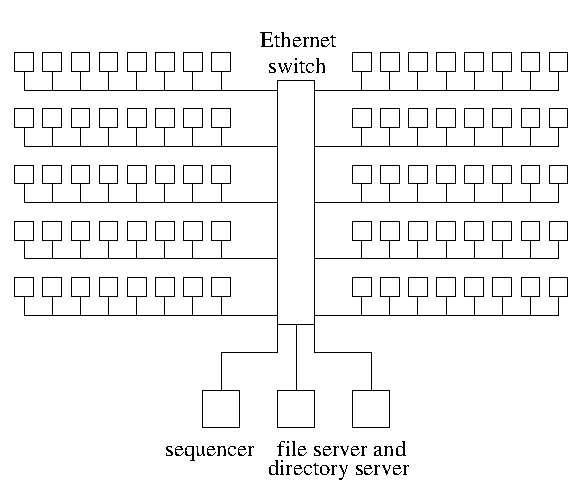
\epsfig{file=PS/zoo.eps,height=5.25cm,width=6cm}
\caption{The Amoeba processor pool}
\label{fig:zoo-pool}
\end{center}
\end{figure}
(see figure~\ref{fig:zoo-pool}).
Each group of eight has its
own 10~Mbit/second channel to an Ethernet switch. Each of the three
additional boards also have their own 10~Mbit/second channel to the Ethernet
switch.

All boards run the Amoeba distributed operating system~\cite{amoeba}. Part
of the Amoeba kernel is the FLIP (Fast Local Internet Protocol~\cite{flip})
network code. All interfaces needed from the host operating system by
the Panda system layer are provided directly in Amoeba. FLIP offers RPC
and group communication and Amoeba offers kernel threads.

\subsection{The Solaris workstations}
Twelve Sun SPARCclassic workstations were used for measurements. All
of these workstations have the same 50~MHz microSPARC processor as
the Amoeba processor pool. They are split in two groups of six and each
group is connected via 10base-2 Ethernet to a repeater
\begin{figure}[htbp]
\begin{center}
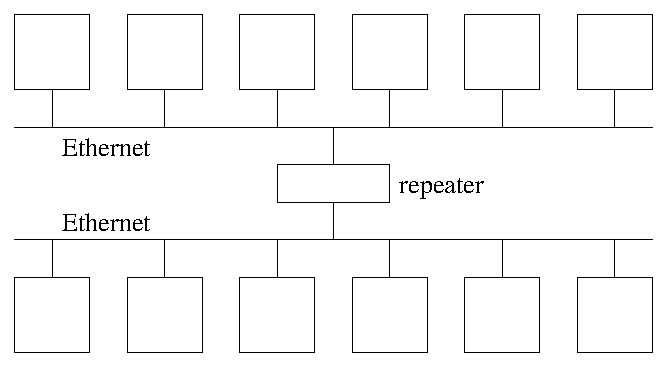
\epsfig{file=PS/sloepen.eps,height=3cm,width=5cm}
\caption{The SPARCclassic LAN}
\label{fig:sloep}
\end{center}
\end{figure}
(see~figure~\ref{fig:sloep}). The workstations
run Solaris~2.4 and have 32~MB RAM. Solaris offers RPC, multicast,
broadcast and kernel threads that can be used directly by the Panda
system layer.

\subsection{The Parix PowerXplorer}
The PowerXplorer is made by Parsytec. It is a
machine with four 80~MHz PowerPC~601 chips.
These chips have a 32~Kb (unified) cache. Each machine has 32~MB~RAM.
Each of the four PowerPCs has a T805 transputer for the communication.
These transputers communicate via 8.8~Mbyte/sec point-to-point links.
The measurements were done on
a collection of eight of these machines. They are interconnected
as shown in 
\begin{figure}[htbp]
\begin{center}
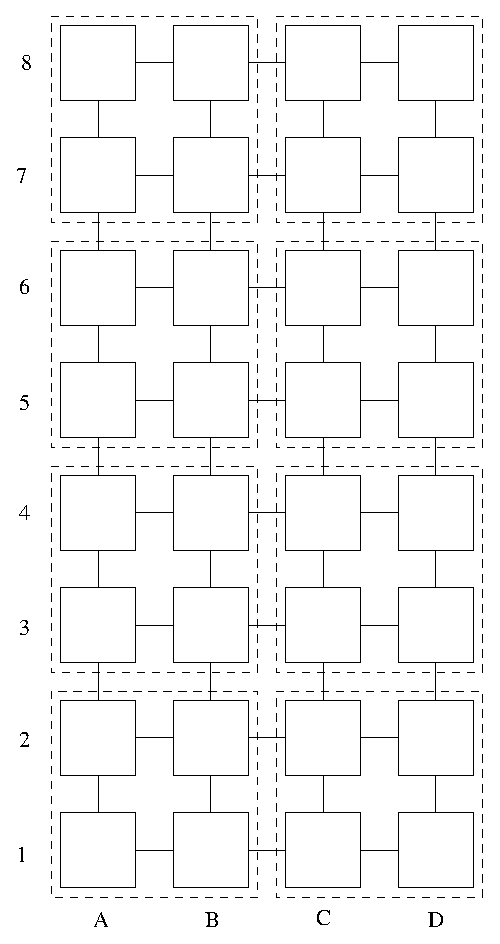
\epsfig{file=PS/ppc-grid.eps,height=8cm,width=4cm}
\caption{The PowerXplorer grid}
\label{fig:ppc-grid}
\end{center}
\end{figure}
figure~\ref{fig:ppc-grid}. The workstations are surrounded by a dashed
box.

The processor grid is divided into several partitions. Each partition is
of rectangular shape (e.g. $1 \times 1,\:3 \times 7$, etc.).
This means it is not possible to run on every
number of processors between 1 and 32. It is easy to see that the
available number of processors is 1 to 10, 12, 14, 15, 16, 18, 20, 21, 24, 28,
and 32.

Because the PowerXplorer grid uses point-to-point links the operations
on replicated objects are implemented differently than on Solaris and Amoeba.
First of all, the point-to-point communication is reliable. So Panda
does not need to send acknowledgements and there is no need to resend
messages. Therefore, the sequencer does not need a buffer for recently
sent messages.

But because the communication is on a point-to-point basis, there is
no broadcast mechanism. Parix does not offer that either. So the Panda
system layer has to implement broadcasting. This is done by building
a spanning tree between all processors~\cite{article:tocs}.
A separate routing daemon
thread on each processor takes care of this. When a broadcast message
is received by a processor, it forwards the message to its neighbours
(except for the neighbour it received the broadcast message from)
on the spanning tree.

Group messages are implemented with an algorithm different from the ones
(PB and BB) used by Solaris and Amoeba. The PB and BB algorithms have
the disadvantage of creating large traffic around the sequencer, because
in both algorithms the sequencer uses broadcasts to send messages or
sequence numbers.
Therefore, on Parix the GSB (Get Sequence number and broadcast) method
is used.
The sender first sends a point-to-point message to the sequencer to
request the current sequence number. The sequencer sends the sequence
number to the sender. Finally, the sender broadcasts the message to
all the other processors. In this case the sequencer only sends 
point-to-point messages and the communication is spread more evenly
over the PowerPC grid.

\section{Implementation of Arc Consistency in Orca}
\label{sec:acp}

The arc consistency program used is based on an existing program written
by I.~Athanasiu and H. E. Bal~\cite{article:irina}.
This program was written partly in
C because at the time it was written, certain parts could not be written
in Orca efficiently. For example, bit operators have been introduced in
the Orca language only recently.
Furthermore, the original program read
the input constraint graph from a file,
which is very slow on Amoeba. These parts of the program
were changed and the resulting
version was used for the measurements presented here. The program is written
entirely in Orca now and the program itself constructs the input
constraint graph. 
Some parameters for constructing the graph are read from standard input.

The arc consistency algorithm used is a parallel version of the {\tt AC-1}
algorithm of figure~\ref{fig:ac-1}.
In the original version the variables were distributed over the processors
using the static load balancing algorithm of J. M. Conrad~\cite{article:conrad}.
This was done by first creating a constraint graph and writing this graph
to a file. The arc consistency program read the graph from the file.
Because the new arc consistency program constructs the constraint graph
in-core, a much simpler distribution was chosen.
A measure for the work to be done is the number of consistency checks to
be done. 
The input graph is constructed in such a way that 
each variable has approximately the same number of constraints.
As a consequence the work to be done per variable is approximately the same
for each variable.
The method used to distribute the load over the processors is to give
each processor approximately the same number of variables.

The parallel
{\tt REVISE} function, called {\tt SPREVISE}, works on a local copy of
the domains of the variables. This is done because working with shared
domains would create too many messages. {\tt SPREVISE} 
returns {\bf true} when the domain of the
variable checked has changed and returns a list of values to be
removed from the domain of the variable. The parallel version of the
{\tt AC-1} function is called {\tt SPAC}.
It uses two major objects, the {\bf domain} object and the {\bf work}
object.
The {\bf domain} object contains the values present in the
domain of each of the variables. The main operations on the {\bf domain}
object are (in pseudo Orca code):
\begin{verbatim}
        domain: [1 .. nr_variables][1 .. nr_values] OF integer;

        OPERATION change(variable, list);
        BEGIN
            FOR i IN list DO
                domain[variable][i] := false;
            OD;
        END;

        OPERATION getvalue(variable): list;
        BEGIN
            RETURN domain[variable];
        END;
\end{verbatim}

The {\bf work} object contains a list of all variables and to which
processor they are assigned. The main operations 
of the {\bf work} object are (in pseudo Orca code):
\begin{verbatim}
        constraint: [1 .. nr_variables][1 .. nr_variables] OF relation_type;
        busy: integer;

        OPERATION announce(variable);
        BEGIN
            needs_checking(variable) := true;
        END;

        OPERATION ready();
        BEGIN
            busy -:= 1;
        END;

        OPERATION init_const();
        BEGIN
            FOR i IN [1 .. nr_variables] DO
                FOR j IN [1 .. nr_variables] DO
                    constraint[i][j] := relation;
                OD;
            OD;
            busy := nr_workers;
        END;

        OPERATION get_const(): graph;
        BEGIN
            RETURN constraint;
        END;

        OPERATION get_work(processor): list;
        BEGIN
            FOR i IN 1 .. nr_variables DO
                IF (on_processor(i) = processor) AND
                            needs_checking(i) THEN
        	    list +:= i;
        	FI;
            OD;
            RETURN list;
        END;
        
        FUNCTION new_work(processor);
        BEGIN
            FOR i IN 1 .. nr_variables DO
                IF (on_processor(i) = processor) AND
                            needs_checking(i) THEN
                    RETURN true;
                FI;
            OD;
            RETURN false;
        END;
\end{verbatim}
\pagebreak
\begin{verbatim}
        FUNCTION any_work();
        BEGIN
            FOR i IN 1 .. nr_variables DO
                IF needs_checking(i) THEN
                    RETURN true;
                FI;
            OD;
        END;
        
        OPERATION work_for(processor): boolean;
        BEGIN
            GUARD new_work(processor) DO
                busy +:= 1;
                RETURN true;
            OD;
        
            GUARD (busy = 0) AND NOT any_work() DO
                RETURN false;
            OD;
        END;
\end{verbatim}

For each variable assigned to
the processor, the {\tt SPAC} function calls {\tt SPREVISE}. If the
domain of the variable was changed, {\tt SPREVISE} updates the shared
object {\bf domain}.
\begin{figure}[htbp]
\begin{center}
\begin{tabbing}
\hspace{2cm} \= \hspace{0.5cm} \= \hspace{0.5cm} \= \hspace{0.5cm}
\= \hspace{0.5cm} \= \\
\> {\bf procedure} {\tt SPREVISE(i, j, domain, value\_list)}: {\bf boolean} \\
\> {\bf begin} \\
\> \> {\tt MODIFIED} = {\bf false} \\
\> \> {\bf for} {\tt each} $x \in D_i$ of domain \\
\> \> {\bf do} \\
\> \> \> {\bf if} {\tt there is no} $y \in D_j$ of domain
{\tt such that} $P_{ij}(x, y)$ \\
\> \> \> {\bf then} \\
\> \> \> \> {\tt value\_list} = {\tt value\_list} $ \cup\:\{x\}$ \\
\> \> \> \> {\tt MODIFIED =} {\bf true} \\
\> \> \> {\bf fi} \\
\> \> {\bf od} \\
\> \> {\bf return} {\tt MODIFIED} \\
\> {\bf end} \\
\\ \\ 
\> {\bf procedure} {\tt SPAC()} \\
\> {\bf begin} \\
\> \> {\tt cpu = MYCPU()} \\
\> \> {\bf repeat} \\
\> \> \> {\bf repeat} \\
\> \> \> \> {\tt CHANGE} = {\bf false} \\
\> \> \> \> {\tt work} = {\tt work\$get\_work(cpu)} \\
\> \> \> \> {\tt domain} = {\tt domain\$get\_value()} \\
\> \> \> \> {\bf for} {\tt each i, j} $\mid P_{ij}(x, y)$ is a constraint \\
\> \> \> \> {\bf do} \\
\> \> \> \> \> {\tt value\_list} = $\{\}$ \\
\> \> \> \> \> {\tt CHANGE} = {\tt REVISE(i, j, domain, value\_list)}
{\bf or} {\tt CHANGE} \\
\> \> \> \> {\bf od} \\
\> \> \> \> {\bf if} {\tt CHANGE} \\
\> \> \> \> {\bf then} \\
\> \> \> \> \> {\tt domain\$change(value\_list)} \\
\> \> \> \> \> {\tt work\$announce(variable)} \\
\> \> \> \> {\bf fi} \\
\> \> \> {\bf until not} {\tt CHANGE} \\
\> \> {\bf until not} {\tt work\$work\_for(cpu)} \\
\> {\bf end}
\end{tabbing}
\caption{The SPREVISE and SPAC functions}
\label{fig:spac}
\end{center}
\end{figure}
In
figure~\ref{fig:spac} the {\tt SPREVISE} and {\tt SPAC} functions are shown.

All workers start with calling the {\tt SPAC} loop. This loop
is run as long as {\tt work\$work\_for} returns true.
This means either there is work to be done or another worker is still
busy.

The implementation of the arc consistency problem was split in two. First,
the constraint graph was constructed. Then, ACP was run on the input data.

The main input data structures are the {\tt constraint} matrix, 
the {\tt relation} matrices and the {\tt domain} matrix.
The {\tt constraint}
matrix is a symmetrical
square matrix with a size of the number of variables. It
indicates whether there is a constraint between two variables. A randomly
chosen {\tt relation} matrix is assigned to each constraint.
The {\tt relation} matrices are symmetrical matrices with the size of the
number of values.
For each pair of values the {\tt relation} matrix indicates whether the
values are in relation with each other.
The {\tt domain} matrix is a matrix of the size of the number of variables
by the number of values. It indicates for every variable which values
are still in its domain.

The program starts with creating these input matrices. One of the input
parameters is the number of constraints per variable. This parameter gives
the number of other variables to which each variable is (randomly) connected.
The seed for the random generator is also one
of the input parameters. In this way the same input matrices will be
generated when the same seed is given. One of the {\tt relation} matrices
is (randomly) assigned to each of the constraints.
The number of relation pairs
per relation is an input parameter. 
The {\tt domain} matrix
is filled with all true values when it is initialised which means that
all variables contain all values at the start of the program.

After the constraint graph is created, the arc consistency part is run
on the graph. For each variable all its values that do not satisfy the
constraints are removed.

\section{Optimisation}
\label{sec:tuning}
In this section some performance optimisations that were applied to the
Orca program of the previous section are described.
Several tools are available for analysing Orca programs. {\em Accounting} gives
information about the operations on shared objects. {\em Profiling} can be used
to get information about the number of calls to all functions
in the program and the time spent on them. Finally, {\em tracing}
gives information
about events, such as starting an operation, blocking on that operation
and continuing after a blocked operation.
All these tools were used to improve the arc consistency program.

Profiling is done on a run of the program on a single processor.
It gives
information that can be analysed with the Unix {\tt prof(1)}
command.
Profiling showed that many {\tt m\_mod} calls were made.
This is a function
of the Orca runtime system that implements the Orca modulo operator.
The cause for these calls were a modulo operation in the {\tt sprevise}
function. The calculation was rewritten as a bit shift calculation. This
reduced the number of {\tt m\_mod} calls dramatically.

Tracing generates files with trace information for each processor.
These trace files can be merged into one trace file
with all events in it. The graphical user interface
{\tt orcshot}~\cite{a:orcshot}) was used to analyse the results.
Several observations were made.
One observation was that the various processors did not start at the
same time
\begin{figure}[htbp]
\begin{center}
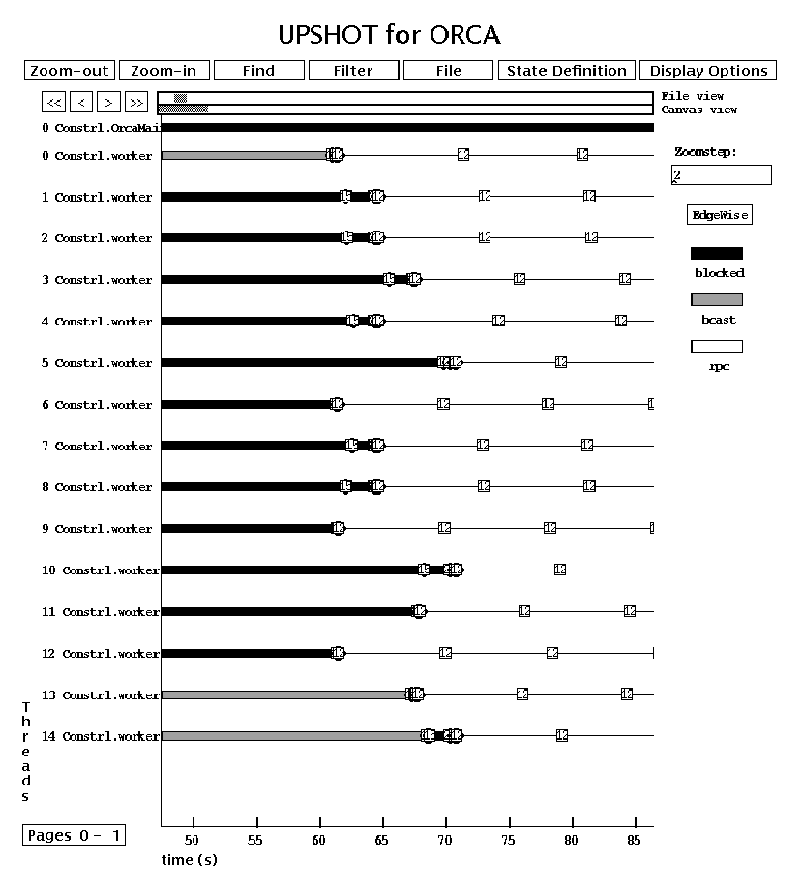
\epsfig{file=PS/start.ps,height=12cm,width=12cm}
\caption{Workers not starting at the same time}
\label{fig:start}
\end{center}
\end{figure}
(see figure~\ref{fig:start}). Horizontal lines correspond to Orca threads.
At the left hand side they are numbered with the processor they run on.
Each event is labeled with a box with a number in it. These boxes correspond
to one or more events, such as blocking, continuing, starting an operation,
etc. When the horizontal line is small, the thread is working. When 
the line is
fat, the thread
is in the state indicated at the right hand side. At the bottom the
time since the program started is shown.

At the left side of the figure all processors are either blocked or
busy sending broadcast messages.
They are all blocked on a {\tt work\$get\_const()} operation
or are busy doing that operation.
The events with label 15 correspond to {\tt work\$get\_work} operations and
thus the start of the {\tt SPAC()} loop. So worker 12 starts its
{\tt SPAC()} loop at around time 52. Worker 5 starts its {\tt SPAC()} loop
only at around time 70. So their is a difference of about 18 seconds.

This was caused by the time it takes to
construct the
constraint matrix in {\tt work\$init\_const}.
Furthermore, at the time {\tt work\$init\_const}
was started, the {\tt work} object was not replicated yet. It was placed
on processor 0 which initialised the {\tt constraint} matrix. This made
the situation even worse. When the other workers called 
{\tt work\$get\_const()}, they got a copy from processor 0. This created
lots of messages.
The code used to be
\begin{verbatim}
    toti$inc();
    IF cpu = 0
    THEN
        work$init_const();
    FI;
    constraint := work$get_const();
    toti$AwaitValue(nr_workers);    # block until toti equals nr_workers
    start := SysMilli();
    SPAC();
    time$Assign(cpu, SysMilli() - start);
\end{verbatim}

The {\tt work} object was not replicated because
{\tt work\$init\_const} was started on
processor~0 at a time when most other workers were still being
started at the other processors. Therefore, the Orca runtime system
could not make
the decision yet to replicate the {\tt work} object. Including a
barrier synchronisation just before {\tt work\$init\_const} made sure
all workers were started and the {\tt work} object was replicated.
Replication was forced by a {\tt Strategy()} call. This is a way
to instruct the runtime system to always replicate an object.

The workers did not start at the same time. This was caused by the fact that
{\tt toti} was incremented before {\tt work\$get\_const()} 
was called. The guard in {\tt toti\$AwaitValue()} would always
be true
when a worker finished its {\tt work\$get\_const()} operation.
When not every worker started 
{\tt work\$get\_const()} at the same time, not every processor would
continue after the guard in {\tt toti\$AwaitValue()} at the
same time. Therefore not every worker started its {\tt SPAC()} loop at the
same time. This was fixed by another barrier synchronisation.
So the code was changed to:
\begin{verbatim}
    sync(bar);
    IF MYCPU() = 0
    THEN
        . . .
        . . .
    FI;
    constraint := work$get_const();
    sync(bar);
    start := SysMilli();
    . . .
    . . .
\end{verbatim}

After these changes all workers started at the same time. But because there
is a synchronisation at the end of the {\tt SPAC()} loop too,
the timing had to be done differently. Instead of getting the
time outside of the {\tt SPAC()} loop, it was done inside the
{\tt SPAC()} loop. The start time is set at the
beginning of the {\tt SPAC()} loop and the finish time is set just before
the call to {\tt work\$Work\_for()} in the {\tt SPAC()} loop. When there is
more work the loop continues. Each time the {\tt SPAC()} loop finishes,
the finish time is set to
the current time at that moment. When finally there is no work anymore the
last value assigned to the finish time is the time that processor finished
its work and started sleeping on the guard in {\tt work\$Work\_for()}.
The difference between the finish time and the start time
is returned as one of the parameters of the {\tt SPAC()} loop.

Tracing also showed a situation where lots of messages were
sent by all workers
\begin{figure}[htbp]
\begin{center}
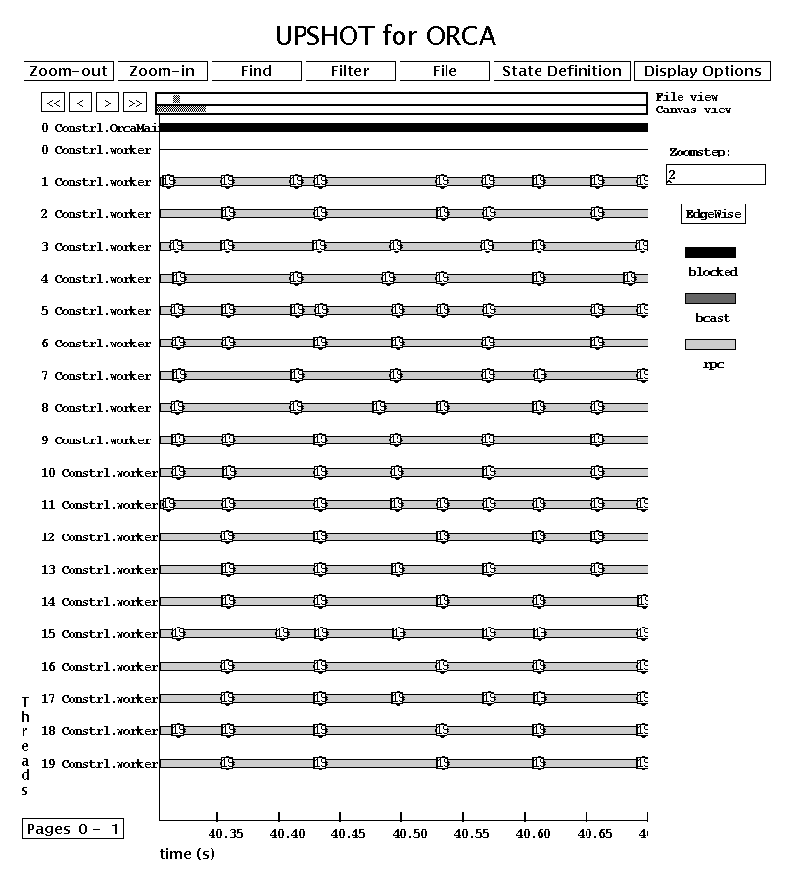
\epsfig{file=PS/trashing.ps,height=12cm,width=12cm}
\caption{Lots of messages being sent by all workers}
\label{fig:trashing}
\end{center}
\end{figure}
(see figure~\ref{fig:trashing}). This was caused by replication decisions
by the runtime system.
The work object started non-replicated, so all workers sent
their operation messages to one processor. But then the runtime system
noticed more
read than write operations on the object and replicated the object. But
it takes some time for the workers to receive the group message in which
the replication is announced. In the mean time all workers still send their
operations to the one processor.
They do not get an acknowledgement, and therefore
resend the message. This generated so many messages that the program
hardly made any progress anymore. This was diagnosed as partially a
bug in the 
runtime system and an unfortunate replication decision by the runtime
system. The program
was changed by inserting a {\tt Strategy()} call, that indicates the objects
should always be replicated.
Orcshot figures~\ref{fig:new-start} and~\ref{fig:new-end} show the
start and end of the {\tt SPAC()} loop of the new version of the program.
Now, the workers start their {\tt SPAC()} loop within
a few tens of a second from each other. The first worker that finishes
its {\tt SPAC()} loop is worker 4. About 5 seconds later the last
worker, number 3, finishes its {\tt SPAC()} loop. So the difference
between the first and the last ready worker is
less than 5\% of the total execution time.
This is an example where tracing proved
to be very helpful in diagnosing bad performance.

\begin{figure}[htbp]
\begin{center}
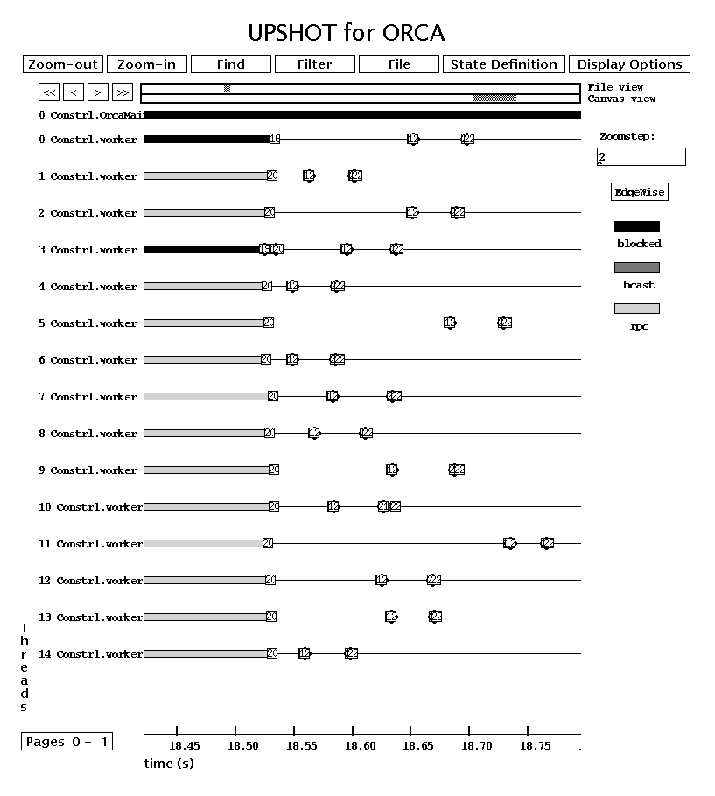
\epsfig{file=PS/new-start.ps,height=12cm,width=12cm}
\caption{Start of {\tt SPAC()} loop}
\label{fig:new-start}
\end{center}
\end{figure}

\begin{figure}[htbp]
\begin{center}
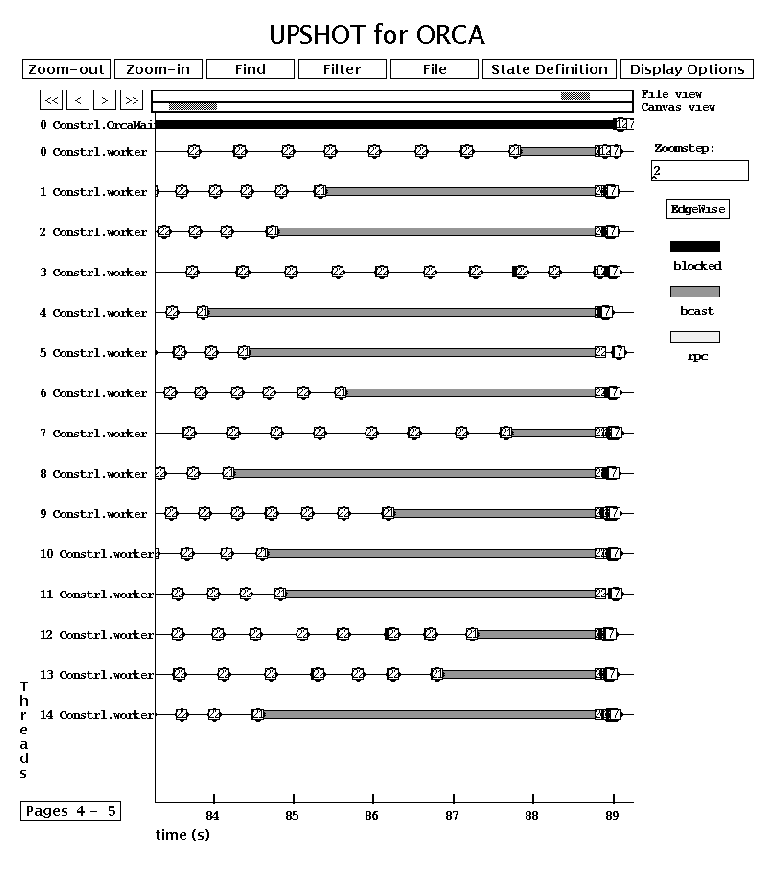
\epsfig{file=PS/new-end.ps,height=12cm,width=12cm}
\caption{End of {\tt SPAC()} loop}
\label{fig:new-end}
\end{center}
\end{figure}

Accounting was used to analyse the number of messages sent by the arc
consistency program. Accounting shows for each shared object the number
of read and write operations. It also shows whether these operations come
from local or remote processes. Furthermore, accounting shows whether an
object is updated by a RPC call (non-replicated object) or by a broadcast
(replicated object). Some results are shown in section~\ref{sec:performance}.

\section{Measurements}
\label{sec:performance}

In this section the performance of the optimised arc consistency program
is discussed. Runs with three different problem sizes
were made on Amoeba, Solaris, and Parix.
Problem sizes 1 to 3
were used for runs on up to 32 processors.
Problem size 1 was also used for a run on up to 72 processors on Amoeba.
It serves as an illustration of the possible speedups
on the Amoeba processor pool. The input data is shown in
\begin{table}[htbp]
\begin{center}
\begin{tabular}{|l|r|r|r|}
\hline
problem size  & 1 & 2 & 3 \\
\hline
nr of variables      & 1000 & 1000 & 1000 \\
nr of values         &  150 &  150 &  150 \\
nr of connections    &  150 &  150 &  150 \\
nr of relations      &    5 &    5 &    5 \\
nr of relation pairs & 1000 &  750 &  500 \\
random seed          &   42 &   42 &   42 \\
\hline
\end{tabular}
\caption{Input data for the three runs}
\label{table:input}
\end{center}
\end{table}
table~\ref{table:input}.
With this input data the number of values removed is 1939 for problem size 1,
22172 for problem size 2 and 149000 for problem size 3.

\begin{figure}[p]
\begin{center}
\epsfig{file=PS/zoo-times.ps,height=5cm,width=8cm}
\caption{Run time on Amoeba}
\label{fig:zoo-times}
\end{center}
\end{figure}

\begin{figure}[p]
\begin{center}
\epsfig{file=PS/sol-times.ps,height=5cm,width=8cm}
\caption{Run time on Solaris}
\label{fig:sol-times}
\end{center}
\end{figure}

\begin{figure}[p]
\begin{center}
\epsfig{file=PS/ppc-times.ps,height=5cm,width=8cm}
\caption{Run time on Parix}
\label{fig:ppc-times}
\end{center}
\end{figure}

\begin{figure}[p]
\begin{center}
\epsfig{file=PS/zoo-speedup.ps,height=5cm,width=8cm}
\caption{Speedups on Amoeba}
\label{fig:zoo-speedup}
\end{center}
\end{figure}

\begin{figure}[p]
\begin{center}
\epsfig{file=PS/sol-speedup.ps,height=5cm,width=8cm}
\caption{Speedup on Solaris}
\label{fig:sol-speedup}
\end{center}
\end{figure}

\begin{figure}[p]
\begin{center}
\epsfig{file=PS/ppc-speedup.ps,height=5cm,width=8cm}
\caption{Speedup on Parix}
\label{fig:ppc-speedup}
\end{center}
\end{figure}

\begin{figure}[p]
\begin{center}
\epsfig{file=PS/zoo-72.ps,height=5cm,width=8cm}
\caption{Speedup on Amoeba of run 4}
\label{fig:zoo-72speedup}
\end{center}
\end{figure}

\begin{table}[H]
\begin{center}
\begin{tabular}{|r|r|r|r|}
\hline
{\bf work}  & total & reads & writes \\
\hline
total & 3267 & 261 & 3006 \\
local &  254 & 254 &    0 \\
BC    & 3013 &   7 & 3006 \\
\hline
\end{tabular}
\end{center}
\caption{Operations on the {\bf work} object}
\label{table:work}
\end{table}

\begin{table}[H]
\begin{center}
\begin{tabular}{|r|r|r|r|}
\hline
{\bf domain}  & total & reads & writes \\
\hline
total & 986 & 3 & 983 \\
local &  3 & 3 &    0 \\
BC    & 983 &   0 & 983 \\
\hline
\end{tabular}
\end{center}
\caption{Operations on the {\bf domain} object}
\label{table:domain}
\end{table}

In
figures~\ref{fig:zoo-times}~-~\ref{fig:ppc-times} the execution times
on Amoeba, Solaris, and Parix are
shown. The corresponding speedups are shown in
figures~\ref{fig:zoo-speedup}~-~\ref{fig:ppc-speedup}.
The speedup of the run of problem size 1 on up to 72 processors
on Amoeba is shown in figure~\ref{fig:zoo-72speedup}.

The speedups on Amoeba and Solaris are better than the speedups on Parix.
One explanation could be  the difference in execution time. On Amoeba and
Solaris the execution times are about three times as high as on Parix.
The total number of operations on shared objects is about the same. 
In tables~\ref{table:work} and~\ref{table:domain} 
the operations on the two major
objects, the {\bf work} object and the {\bf domain} object,
are shown. These numbers are
from a run on eight processors with problem size 1. The total number of
operations on the {\bf work} object is 3267. 3006 of them
are write operations, 261 are
read operations. All write operations are broadcasts, because the {\bf work}
object is replicated. The read operations can be done locally.

The seven broadcast reads are an interesting case.
The {\tt work\_for()} operation has two guards. One of the guards represents
a write operation, the other guard represents a read operation.
\begin{verbatim}
        OPERATION work_for(processor): boolean;
        BEGIN
            GUARD new_work(processor)
            DO
                busy +:= 1;
                RETURN true;
            OD;
        
            GUARD (busy = 0) AND NOT any_work()
            DO
                RETURN false;
            OD;
        END;
\end{verbatim}
Because the operation is a possible write operation, it will be
broadcast. When the operation continues because the read guard is
satisfied, the operation is counted as a (broadcast) read.

Just before calling {\tt work\_for()} the worker calls
{\tt work\_ready()}. This operation decreases {\tt busy} by one.
For all but the last worker, {\tt busy} will be greater than zero
when {\tt work\_for()} is called and the guard blocks on {\tt any\_work()}.
When the last worker calls {\tt work\_for()}, {\tt busy = 0} and
the read guard in {\tt work\_for()} is immediately satisfied. So the
operation can be done locally for the last worker. For all other
workers the read guard in {\tt work\_for()} is satisfied too. So all
continue and the operation counts as a broadcast read. That is why
there are seven broadcast reads when the program is run on eight
processors.

From the table above it can be seen that the total number of
operation messages is about 4000. On 10 processors
the program takes about 200 seconds on Amoeba and
Solaris. On Parix it takes about 90 seconds.
This means on Amoeba and Solaris about 20 messages per second are sent.
On Parix about 44 messages are sent each second.
Therefore, on Parix the communication overhead is larger than
on Amoeba or Solaris. This decreases the speedup.

\begin{figure}
\begin{center}
\epsfig{file=PS/zoo.con_checks.ps,height=5cm,width=8cm}
\caption{Total number of consistency checks}
\label{fig:zoo-con-checks}
\end{center}
\end{figure}

\begin{figure}
\begin{center}
\epsfig{file=PS/zoo.checks.per.processor.ps,height=5cm,width=8cm}
\caption{Number of consistency checks per processor}
\label{fig:zoo-checks-per-processor}
\end{center}
\end{figure}

In
figure~\ref{fig:zoo-checks-per-processor} the number of consistency checks
per processor of the three runs on Amoeba is shown.

The number of consistency checks is a good measure for the
work done. Figure~\ref{fig:zoo-con-checks} shows the total number of
consistency checks. The number of consistency checks per processor is
shown in figure~\ref{fig:zoo-checks-per-processor}. Both are from runs
on Amoeba.

For problem size 1 the total number of consistency
checks is the same regardless of the number of 
processors used to run the program on.

For problem size 3 the total number of consistency checks
increases with the number of 
processors. So when more processors are used to run the program, they
are doing redundant work. This can be explained by the number of values
removed. For problem size 3 the number of values removed is about
100 times the
amount for problem size 1. Because updates on the {\bf domain} object are not
done immediately, other processors may be checking values that are
already removed by other processors.

The number of consistency checks for problem size 2 is the largest of the
three. This corresponds to the fact that it has also the largest
execution times. The number of consistency checks on a single
processor run is about 40\% lower than that of runs on a larger number of
processors. Therefore, the speedup is worse than the speedup of problem
size 1.

\section{Conclusions}
\label{sec:discussion}
In this thesis an implementation of the arc consistency program in Orca
has been discussed. It is not difficult to learn Orca. Most language
constructs are similar to other languages, like Modula-2. The shared
data-object model has proven to be an easy to understand and use paradigm.
It makes writing parallel programs comparatively easy, because the
programmer does not need to concentrate on communication mechanisms
between the processors. The shared data-object model takes care of this.

But in order to write programs that achieve good speedups, the programmer
has to be aware of the way Orca is implemented. For example, the arc
consistency problem works with a set of variables. Although Orca has
the {\tt set} type, nobody uses it because its current implementation
is too slow.

{\em Orcshot} has proven to be a useful tool to analyse Orca programs.
It is attractive to be able to view all operations on all
processors and see why a processor is blocked at a certain time.
But unfortunately, to be able to interpret the information correctly,
a thorough knowledge of the working of the runtime system is necessary.

The arc consistency program showed good speedups on Amoeba and Solaris.
On Amoeba a speedup of about 65\% on 72 processors was achieved. On 32
processors the speedup is about 89\%. On solaris the speedup is about
92\% on 12 processors. On Parix the speedup was much lower. On 32
processors the speedup is only 40\%.
However, the PowerPC processors in the PowerXplorer are faster than the
SPARC processor used on Amoeba and Solaris. The runs on Amoeba and
Solaris are about three times as slow as on Parix.
This means the communication overhead on Parix is higher and therefore
the speedups are expected to be lower.
Usually, to compensate for faster processors a larger problem size is chosen.
Unfortunately, the arc consistency program is very sensitive
with regard to its input parameters and it takes a lot of time time come
up with a good set of input parameters. Therefore, no fourth problem
size was investigated.

\section{Acknowledgements}
I would like to thank the members of the Orca group for their useful
discussions. Ceriel Jacobs has told me much about the way Orca constructs
are implemented. Rutger Hofman and Koen Langendoen were always there
to explain the details of Panda and the runtime system to me.
I was often surprised how quickly they would find bugs in
Panda and the Orca runtime system and fix them.
With Koen I had many useful discussions about the arc consistency
program.
Finally, I wish to thank Henri Bal for the pleasant and enthusiastic
supervision.

\bibliographystyle{plain}
\bibliography{thesis}

\end{document}
